\documentclass[12pt]{extarticle}
%%%%%%%%%%%%%%% PACKAGES %%%%%%%%%%%%%%%
\usepackage{titleps}
\usepackage{url}
\usepackage{amsmath}
\usepackage{cancel}
\usepackage{amsfonts}
\usepackage{booktabs}
\usepackage{amssymb}
\usepackage{mathtools}
\usepackage{graphicx}
\usepackage[dvipsnames]{xcolor}
\usepackage[colorlinks]{hyperref}
\usepackage{geometry}
\geometry{
    a4paper,
    left=19mm,
    right=19mm,
    top=20mm,
    bottom=25mm
}
% Define dark and mid color

\definecolor{Sepia}{HTML}{704214}
\definecolor{RedViolet}{HTML}{C71585}

\hypersetup{
	colorlinks=true,
	linkcolor=Golden,
    linkcolor=Golden,
    filecolor=Golden,
    citecolor = Golden,
    urlcolor=Golden, % change this to your desired color
}

% Mix lighter shade

\colorlet{LightSepia1}{Sepia!80!yellow}
\colorlet{LightSepia2}{Sepia!70!orange}
\colorlet{DarkGolden}{RedViolet!30!yellow!70!Maroon!70!Brown}
\colorlet{Golden}{RedViolet!30!yellow!70!pink!90!Brown}
\colorlet{DDarkGolden}{RedViolet!20!yellow!70!Maroon!70!Black!65!Brown}

%%%%%%%%%%%%%%%%%%%%%%%%%%%%%%%%%%%%%%%%
%%%%%%%%%%%%%%% FONT %%%%%%%%%%%%%%%%%%%
\usepackage[T1]{fontenc}
\usepackage{charter}

\def\primarycolor{DarkGolden}
\def\secondarycolor{Golden}
%%%%%%%%%%%%%%%%%%%%%%%%%%%%%%%%%%%%%%%%
%%%%%%%%%%%%%%% HEADER %%%%%%%%%%%%%%%%%
\usepackage{fancyhdr}
\let\oldheadrule\headrule
\renewcommand{\headrule}{\color{\secondarycolor}\oldheadrule}
\renewcommand{\headrulewidth}{0.7pt}
\pagestyle{fancy}
\fancyhead{}\fancyfoot{}
\fancyhead[L]{\scshape \large \color{\primarycolor}{\fontfamily{qpl}\selectfont
Amirreza "Farnam" Taheri \\
Student ID: 4021300198003
}}
\fancyhead[R]{\color{\secondarycolor}}
\fancyfoot[C]{\textcolor{\primarycolor}{(\thepage)}}
\setlength{\headheight}{1cm}

\fancypagestyle{headerpage}{
    \fancyhf{} % Clear header and footer
    \renewcommand{\headrulewidth}{0pt} % Remove header rule
    \renewcommand{\footrulewidth}{0pt} % Remove footer rule
    \fancyhead[R]{} % Remove the line that displays "Course Name (Course Code)" in the header page
}

%%%%%%%%%%%%%%%%%%%%%%%%%%%%%%%%%%%%%%%%
%%%%%%%%%%%%%%% COMMANDS %%%%%%%%%%%%%%%
% \newcommand{\norm}[1]{\lVert#1\rVert}
% \newcommand{\inner}[1]{\langle#1\rangle}
\newcommand{\problem}[1]{
    \subsection*{\textcolor{\secondarycolor}{#1}}
    \addcontentsline{toc}{subsection}{\protect\numberline{}#1}
}
\newcommand{\partof}[1]{
    \subsubsection*{\textcolor{\secondarycolor}{(#1)}}
    \addcontentsline{toc}{subsubsection}{\protect\numberline{}#1}
}
\newcommand{\imp}{\implies}
\newcommand{\rond}[2]{\frac{\partial #1}{\partial #2}}
\newcommand{\drond}[2]{\dfrac{\partial #1}{\partial #2}}
\newcommand{\norm}[1]{\lvert#1\rvert}
\newcommand{\expec}[1]{\mathbb{E}\left(#1\right)}
\newcommand{\var}[1]{\mathrm{Var}\left(#1\right)}
\newcommand{\cov}[1]{\mathrm{Cov}\left(#1\right)}
\newcommand{\prob}[1]{\mathbb{P}\left(#1\right)}
\newcommand{\ones}{$\star$}
\newcommand{\twos}{$\star\star$}
\newcommand{\threes}{$\star\star\star$}
\newcommand{\fours}{$\star\star\star\star$}
%%%%%%%%%%%%%%%%%%%%%%%%%%%%%%%%%%%%%%%%
%%%%%%%%%%%%%%% BODY %%%%%%%%%%%%%%%%%%%
\linespread{1.4}
\color{DDarkGolden}
\begin{document}
\setlength{\abovedisplayskip}{6pt}
\setlength{\belowdisplayskip}{6pt}
\setlength{\abovedisplayshortskip}{0pt}
\setlength{\belowdisplayshortskip}{0pt}
%%%%%%%%%%%%%%% CONTENT %%%%%%%%%%%%%%%%
\thispagestyle{headerpage} % Apply custom header style to this page only
\begin{center}
    \vspace*{1.5cm}
    {\Huge\bfseries\color{\primarycolor}{\fontfamily{qpl}\selectfont Project 1: Real Bussiness Cycles}} \\
    \vspace{3cm}
    
\includegraphics[width=6cm]{teias.png} \\ % Replace "university_logo.png" with the actual filename of your university logo
    \vspace{2cm}
    {\Large\color{\primarycolor}{\fontfamily{qpl}\selectfont Amirreza "Farnam" Taheri}} \\
    {\large\color{\primarycolor}{Student ID: 4021300198003}} \\
    \vspace{3cm}
    {\large\bfseries\color{\secondarycolor}{Macroeconomics I}} \\
    \vspace{1cm}
    {\large\color{\secondarycolor}{Instructor: Prof. Hosein Joshaghani}} \\
    \vspace{3cm}
    {\large\color{\secondarycolor}{May 11, 2024}} % Replace with the actual date or semester information
\end{center}
\newpage % Add a page break after the header page

%%%%%%%%%%%%%%% CONTENT %%%%%%%%%%%%%%%%
\pagestyle{fancy} % Apply fancy header to the remaining pages
\fancyhead[R]{\color{\secondarycolor} Project1 - RBC} % Display "Problemset #no" in the header of the remaining pages
%%%%%%%%%%%%%%%%%%%%%%%%%%%%%%%%%%%%%%%%
%%%%%%%%%%%%%%%%%%%%%%%%%%%%%%%%%%%%%%%%
\problem{1. Solve and Log-Linearize}
Find equations describing the system. Find the steady state values of control and state parameters for
this economy.
\partof{Household's Problem}
The representative household maximizes its lifetime utility function subject to it budget constraint:
   \begin{align}
    \underset{c_t,k_{t+1}, N_t}{\max}\quad U &= \mathbb{E}_t \left[ \sum_{i=0}^{\infty} \beta^{t} \left(\log c_t - AN_t \right) \right]\\
    \text{s.t.  }\quad c_t + k_{t+1} &\leq w_t N_t + (1 + R_t - \delta) k_t + \Pi_t
   \end{align}\\
The Lagrangian for household problem is:
\begin{equation}
    \mathcal{L}= \mathbb{E}_t\sum_{i=0}^{\infty} \beta^{t} \left[  \left( \log c_t - AN_t \right)
    -\mu_{t}\left( c_t + k_{t+1} - w_t N_t - (1 + R_t - \delta) k_t  \right)\right]
\end{equation} \\\\
The FOCs are:
\begin{align}
    \dfrac{\partial \mathcal{L}}{\partial c_{t}} &= \frac{1}{c_t} - \mu_{t} = 0\\
    \dfrac{\partial \mathcal{L}}{\partial N_{t}} &= A - \mu_{t}w_t = 0\\
    \dfrac{\partial \mathcal{L}}{\partial k_{t+1}} &= \beta\; \mathbb{E}\{\mu_{t+1}(1 + R_t - \delta)\} - \mu_{t}  = 0 
\end{align}\\
Substituting equation (4) into the equation (5), we get:
\begin{equation}
    {A}c_t = {w_t}
\end{equation}\\
Substituting equation (4) into the equation (6), we get:
\begin{equation}
    \beta\; \mathbb{E}\{\frac{1}{c_{t+1}}(1 + R_t - \delta)\} = \frac{1}{c_t}
\end{equation}\\
\newpage
%%%%%%%%%%%%%%%%%%%%%%%%%%%%%%%%%%%%%%%%
\partof{Firm's Problem}
The firm's technology is described by the production function:
    \begin{equation}
    Y_t = z_t k_t^{\alpha} N_t^{1-\alpha}
   \end{equation} \\
The technology follows an $AR1$ process:
    \begin{equation}
    \log(z_{t+1}) = \rho \log(z_t) + \epsilon_t, \quad \epsilon_t \sim IID
   \end{equation} \\
Firm wants to maximize its profit:
\begin{equation}
    \max\quad \Pi_t = z_t k_t^{\alpha} N_t^{1-\alpha} - w_t N_t - R_t k_t 
   \end{equation}\\
The optimality conditions are:
   \begin{align}
        MP_L &= (1-\alpha) z_t k_t^{\alpha} N_t^{-\alpha} = w_t\\
        MP_K &= \alpha\; z_t k_t^{\alpha-1} N_t^{1-\alpha} = R_t
    \end{align}\\\\
The structural equations of the economy are:
\begin{align}
    \textsc{(LNS,\;Market Clearing)}&\qquad c_t + k_{t+1} = w_t N_t + (1 + R_t - \delta) k_t + \Pi_t\\
    \textsc{(Production of Economy)}&\qquad \qquad \;\;\;Y_t = z_t k_t^{\alpha} N_t^{1-\alpha}
\end{align}
    
\newpage
%%%%%%%%%%%%%%%%%%%%%%%%%%%%%%%%%%%%%%%%
\partof{The Steady State}
\setcounter{equation}{0}
In the steady state we have no shock and zero profit $(\Pi=0,\;z=1)$.
Also the sytem parameters has no dynamic. So the equations are:\\
$$\textbf{Supply:}$$
\begin{align*}
    {A}c &= {w}\\
    \implies w&={3}{c}\\\\
    \beta\; \frac{1}{c}(1 + R - \delta) &= \frac{1}{c} \\
    \implies R&=\dfrac{1}{\beta}+\delta-1\\
    \implies R&=\dfrac{1}{0.99}+0.025-1 =  0.035\; \checkmark
\end{align*}\\
$$\textbf{Demand:}$$
\begin{align*}
    (1-\alpha)\; k^{\alpha} N^{-\alpha} &= w\\
    \implies (1-0.36)\; k^{0.36} N^{-0.36} &= w \tag{i}\\\\
    \alpha\; k^{\alpha-1} N^{1-\alpha} &= R\\
    \implies 0.36\; k^{0.36-1} N^{1-0.36} &= 0.035 \tag{ii}
\end{align*}\\
$$\textbf{Structural equations:}$$
\begin{align*}
    c &= w N + (R - \delta) k\\
    \dfrac{w}{3} &= w N + (0.035 - 0.025) k \tag{iii}\\\\
    Y &= k^{\alpha} N^{1-\alpha}\\
\end{align*}\\
From (i), (ii) we get:
\begin{align*}
    \dfrac{k}{N}=38,\;w=2.37 \tag{iv}
\end{align*}\\
From (iii), (iv) we get:
\begin{align*}
    k=10.9,\;N=0.28 \tag{v}
\end{align*}\\
From (v) and production function, we get:
\begin{align}
    y=1.06 \tag{vi}
\end{align}\\
From (iv), $w={3}{c}$, we get:
\begin{align*}
    c=0.79 \tag{vii}
\end{align*}\\
From (v) and law of motion of capital, $0=k(-\delta)+i$, we get:
\begin{align*}
    i=0.27
\end{align*}

\newpage
%%%%%%%%%%%%%%%%%%%%%%%%%%%%%%%%%%%%%%%%
%%%%%%%%%%%%%%%%%%%%%%%%%%%%%%%%%%%%%%%%
\problem{2. Log-Linearization}
\setcounter{equation}{0}
$$\textbf{Supply:}$$
\begin{align}
    c_t = {A}{w_t}\\
    \beta\; \mathbb{E}\{\frac{1}{c_{t+1}}(1 + R_t - \delta)\} = \frac{1}{c_t}
\end{align}\\
$$\textbf{Demand:}$$
\begin{align}
    (1-\alpha) z_t k_t^{\alpha} N_t^{-\alpha} &= w_t\\
    \alpha\; z_t k_t^{\alpha-1} N_t^{1-\alpha} &= R_t
\end{align}\\   
$$\textbf{Structural equations:}$$
\begin{align}
    Y_t &= c_t + i_t \\
    Y_t &= z_t k_t^{\alpha} N_t^{1-\alpha}\\
    \log(z_{t+1}) &= \rho \log(z_t) + \epsilon_t\\
    k_{t+1} &= k_t(1-\delta) + i_t
\end{align}\\
Log-linearizing (1), we get:
\setcounter{equation}{0}
\renewcommand{\theequation}{\roman{equation}}
%%%%%%%%%%%%%%%%%%%%%%%%%%%%%%%%%%%%
\begin{equation}
    \tilde{c}_t=\tilde{w}_t
\end{equation}\\
%%%%%%%%%%%%%%%%%%%%%%%%%%%%%%%%%%%%
Log-linearizing (2), we get:
\begin{equation}
    \expec{\tilde{c}_{t+1}}=\beta\expec{\tilde R_{t+1}}+\tilde{c}_t
\end{equation}\\
%%%%%%%%%%%%%%%%%%%%%%%%%%%%%%%%%%%%
Log-linearizing (3), we get:
\begin{equation}
    \tilde{z}_t+\alpha \tilde{k}_t -\alpha \tilde{N}_t=\tilde{w}_t
\end{equation}\\
%%%%%%%%%%%%%%%%%%%%%%%%%%%%%%%%%%%%
Log-linearizing (4), we get:
\begin{equation}
    \tilde{z}_t+(\alpha-1) \tilde{k}_t -(\alpha-1) \tilde{N}_t=\expec{\tilde{R}_{t+1}}
\end{equation}\\
%%%%%%%%%%%%%%%%%%%%%%%%%%%%%%%%%%%%
Log-linearizing (5), we get:
\begin{equation}
    \tilde Y = \dfrac{c}{Y} \tilde{c}_t+ \dfrac{i}{Y} \tilde{i}_t
\end{equation}\\
%%%%%%%%%%%%%%%%%%%%%%%%%%%%%%%%%%%%
Log-linearizing (6), we get:
\begin{equation}
    \tilde{Y}_t=\alpha \tilde{k}_t + (1-\alpha) \tilde{N}_t
\end{equation}\\
%%%%%%%%%%%%%%%%%%%%%%%%%%%%%%%%%%%%
Log-linearizing (7), we get:
\begin{equation}
    \tilde{z}_{t+1}=\rho \tilde{z}_t
\end{equation}\\
%%%%%%%%%%%%%%%%%%%%%%%%%%%%%%%%%%%%
Log-linearizing (8), we get:    
\begin{equation}
    \tilde{k}_{t+1}=(1-\delta)\tilde{k}_t+\delta \tilde{i}_t
\end{equation}

\newpage
%%%%%%%%%%%%%%%%%%%%%%%%%%%%%%%%%%%%%%%%
%%%%%%%%%%%%%%%%%%%%%%%%%%%%%%%%%%%%%%%%
\problem{2. Linear Rational Expectation Model}
\setcounter{equation}{0}
\renewcommand{\theequation}{\roman{equation}}
%%%%%%%%%%%%%%%%%%%%%%%%%%%%%%%%%%%%
\begin{equation}
    \tilde{z}_t=\dfrac{\tilde{z}_{t+1}}{\rho}
\end{equation}\\
%%%%%%%%%%%%%%%%%%%%%%%%%%%%%%%%%%%%
\begin{equation}
    \tilde{c}_t=\beta\expec{\tilde R_{t+1}}-\expec{\tilde{c}_{t+1}}
\end{equation}\\
%%%%%%%%%%%%%%%%%%%%%%%%%%%%%%%%%%%%
\begin{equation}
    \tilde{w}_t=\tilde{c}_t=\beta\expec{\tilde R_{t+1}}-\expec{\tilde{c}_{t+1}}
\end{equation}\\\\

%%%%%%%%%%%%%%%%%%%%%%%%%%%%%%%%%%%%
$$\begin{Bmatrix}
    \tilde Y_t = \dfrac{c}{Y} \beta\expec{\tilde R_{t+1}}-\expec{\tilde{c}_{t+1}}+ \dfrac{i}{Y} \left[\dfrac{1}{\delta}\tilde{k}_{t+1}-\dfrac{1-\delta}{\delta}\tilde{k}_t\right] \hfill\\
    \begin{rcases}
        \tilde{Y}_t=\alpha (\tilde{k}_t - \tilde{N}_t) +  \tilde{N}_t\\
        \alpha \left(\tilde{k}_t - \tilde{N}_t\right)=\beta\expec{\tilde R_{t+1}}-\expec{\tilde{c}_{t+1}} - \dfrac{\tilde{z}_{t+1}}{\rho}
    \end{rcases} \implies \tilde{Y}_t=\beta\expec{\tilde R_{t+1}}-\expec{\tilde{c}_{t+1}} - \dfrac{\tilde{z}_{t+1}}{\rho} +  \tilde{N}_t
\end{Bmatrix}$$\\
$$\begin{rcases}
    \implies    \tilde{N}_t + \dfrac{i}{Y} \left[\dfrac{\delta-1}{\delta}\right]\tilde{k}_t= (\dfrac{c}{Y} -1) \beta\expec{\tilde R_{t+1}} + \dfrac{i}{Y} \left[\dfrac{1}{\delta}\tilde{k}_{t+1}\right]+ \dfrac{\tilde{z}_{t+1}}{\rho}\\
    \hfill \tilde{z}_t+(\alpha-1) \tilde{k}_t -(\alpha-1) \tilde{N}_t=\expec{\tilde{R}_{t+1}} 
\end{rcases}$$\\
\setcounter{equation}{0}
\renewcommand{\theequation}{\arabic{equation}}
%%%%%%%%%%%%%%%%%%%%%%%%%%%%%%%%%%%%
\setcounter{equation}{0}
\renewcommand{\theequation}{\roman{equation}}
%%%%%%%%%%%%%%%%%%%%%%%%%%%%%%%%%%%%
\begin{align}
    \tilde{c}_t=\tilde{w}_t
\end{align}
%%%%%%%%%%%%%%%%%%%%%%%%%%%%%%%%%%%%
\begin{align}
    \expec{\tilde{c}_{t+1}}=0.99\expec{\tilde R_{t+1}}+\tilde{c}_t
\end{align}
%%%%%%%%%%%%%%%%%%%%%%%%%%%%%%%%%%%%
\begin{align}
    \tilde{z}_t+ 0.36 \tilde{k}_t - 0.36 \tilde{N}_t=\tilde{w}_t
\end{align}
%%%%%%%%%%%%%%%%%%%%%%%%%%%%%%%%%%%%
\begin{align}
    \tilde{z}_t+(0.36-1) \tilde{k}_t -(0.36-1) \tilde{N}_t=\expec{\tilde{R}_{t+1}}
\end{align}
%%%%%%%%%%%%%%%%%%%%%%%%%%%%%%%%%%%%
\begin{align}
    \tilde Y_t = \dfrac{0.79}{1.06} \tilde{c}_t+ \dfrac{0.27}{1.06} \tilde{i}_t
\end{align}
%%%%%%%%%%%%%%%%%%%%%%%%%%%%%%%%%%%%
\begin{align}
    \tilde{Y}_t=0.36 \tilde{k}_t + (1-0.36) \tilde{N}_t
\end{align}
%%%%%%%%%%%%%%%%%%%%%%%%%%%%%%%%%%%%
\begin{align}
    \tilde{z}_{t+1}=0.95 \tilde{z}_t
\end{align}
%%%%%%%%%%%%%%%%%%%%%%%%%%%%%%%%%%%%
\begin{align}
    \expec{\tilde{k}_{t+1}}-(1-0.025)\tilde{k}_t = 0.025 \tilde{i}_t
\end{align}\\
\begin{align*}
    (i,ii,iii,vii) \implies&  0.36 \tilde{k}_t - 0.36 \tilde{N}_t=\expec{\tilde{c}_{t+1}}-0.99\expec{\tilde R_{t+1}}- \dfrac{\expec{\tilde z_{t+1}}}{0.95}\\
    (ii,v,vi) \implies&  \dfrac{0.79}{1.06} (\expec{\tilde{c}_{t+1}}-0.99\expec{\tilde R_{t+1}})+ \dfrac{0.27}{1.06} \dfrac{\expec{\tilde{k}_{t+1}}-(1-0.025)\tilde{k}_t}{0.025} = 0.36 \tilde{k}_t + (0.64) \tilde{N}_t \hfill\\
    (vii) \implies &    \tilde{z}_{t+1}=0.95 \tilde{z}_t\\
    (ii) \implies &     \expec{\tilde{c}_{t+1}}=0.99\expec{\tilde R_{t+1}}+\tilde{c}_t
\end{align*}\\
Solving the system with Python (\textbf{\href{run:System Solver.ipynb}{Click Here to Open}}), we get:
\begin{align}
    \tilde k_t &= -0.228\expec{R_{t+1}} + 0.231\expec{c_{t+1}} + 0.932\expec{k_{t+1}} - 0.171\expec{z_{t+1}}\\
    \tilde N_t &= 2.522\expec{R_{t+1}} - 2.547\expec{c_{t+1}} + 0.932\expec{k_{t+1}} + 2.753\expec{z_{t+1}}
\end{align}

\begin{align}
    \tilde{z}_t&=1.053\expec{\tilde{z}_{t+1}}\\
    \tilde{c}_t&=-0.990\expec{\tilde R_{t+1}}+\expec{\tilde{c}_{t+1}}
\end{align}

\newpage

%%%%%%%%%%%%%%%%%%%%%%%%%%%%%%%%%%%%%%%%

Let:
$$\tilde{X}_t = \begin{bmatrix} \tilde{k}_t \\ \tilde{N}_t \\ \tilde{z}_t \\ \tilde{c}_t \end{bmatrix}$$

Then, we can rewrite the system as:
$$\begin{bmatrix} 1 & 0 & 0 & 0 \\ 0 & 1 & 0 & 0 \\ 0 & 0 & 1 & 0 \\ 0 & 0 & 0 & 1 \end{bmatrix} \begin{bmatrix} \tilde{k}_t \\ \tilde{N}_t \\ \tilde{z}_t \\ \tilde{c}_t \end{bmatrix} = \begin{bmatrix} -0.228 & 0.231 & 0.932 & -0.171 \\ 2.522 & -2.547 & 0.932 & 2.753 \\ 0 & 0 & 1.053 & 0 \\ -0.990 & 1 & 0 & 1 \end{bmatrix} \begin{bmatrix} \expec{\tilde{k}_{t+1}} \\ \expec{\tilde{N}_{t+1}} \\ \expec{\tilde{z}_{t+1}} \\ \expec{\tilde{c}_{t+1}} \end{bmatrix}$$

Multiplying both sides by $I_4^{-1}$ from left:
$$\begin{bmatrix} \tilde{k}_t \\ \tilde{N}_t \\ \tilde{z}_t \\ \tilde{c}_t \end{bmatrix} = \begin{bmatrix} 1 & 0 & 0 & 0 \\ 0 & 1 & 0 & 0 \\ 0 & 0 & 1 & 0 \\ 0 & 0 & 0 & 1 \end{bmatrix}^{-1} \begin{bmatrix} -0.228 & 0.231 & 0.932 & -0.171 \\ 2.522 & -2.547 & 0.932 & 2.753 \\ 0 & 0 & 1.053 & 0 \\ -0.990 & 1 & 0 & 1 \end{bmatrix} \begin{bmatrix} \expec{\tilde{k}_{t+1}} \\ \expec{\tilde{N}_{t+1}} \\ \expec{\tilde{z}_{t+1}} \\ \expec{\tilde{c}_{t+1}} \end{bmatrix}$$

Simplifying, we get:
$$\tilde{X}_t = \begin{bmatrix} -0.228 & 0.231 & 0.932 & -0.171 \\ 2.522 & -2.547 & 0.932 & 2.753 \\ 0 & 0 & 1.053 & 0 \\ -0.990 & 1 & 0 & 1 \end{bmatrix} \expec{\tilde{\mathbf{X}}_{t+1}}$$
So $A^{-1}B$ is:
$$A^{-1}B = \begin{bmatrix} -0.228 & 0.231 & 0.932 & -0.171 \\ 2.522 & -2.547 & 0.932 & 2.753 \\ 0 & 0 & 1.053 & 0 \\ -0.990 & 1 & 0 & 1 \end{bmatrix}$$
\newpage
\setcounter{equation}{0}
\renewcommand{\theequation}{\arabic{equation}}
%%%%%%%%%%%%%%%%%%%%%%%%%%%%%%%%%%%%%%%%
%%%%%%%%%%%%%%%%%%%%%%%%%%%%%%%%%%%%%%%%
\problem{3. Eigen-values}

Running the MATLAB code (\textbf{\href{run:eigenvalues.m}{Click Here to Open}}), we will reach to the following eigenvalues:
\begin{align}
    \lambda_1&=-3.4346\\
    \lambda_2&=0.0007\\
    \lambda_3&=1.6590\\
    \lambda_4&=-1.0530
\end{align}
The only eigenvalue satisfying $|\lambda|<1$ is $\lambda_2=0.00067497$, which is corresponding with:
$$\vec{v}_2=\begin{bmatrix}
    0.71066     &0.70353           &0  &2.6584e-05
\end{bmatrix}$$\\
\newpage
\setcounter{equation}{0}
\renewcommand{\theequation}{\arabic{equation}}
%%%%%%%%%%%%%%%%%%%%%%%%%%%%%%%%%%%%%%%%
%%%%%%%%%%%%%%%%%%%%%%%%%%%%%%%%%%%%%%%%
\problem{4. Dynare}
$$\textbf{To open the Dynare script for this problem: \href{run:Farnam_RBC.mod}{Click Here}}$$\\
Here are \LaTeX\; output of the Dynare model.\\
\begin{table}[h]
    \caption{Endogenous Variables}
    \centering
    \begin{tabular}{ccc}
    \hline
    \textbf{Variable} & \textbf{\LaTeX} & \textbf{Description} \\
    \hline\hline
    Y & $Y$ & Output \\
    I & $I$ & Investment \\
    K & $K$ & Capital \\
    N & $N$ & Labor \\
    A & $A$ & Technology \\
    C & $C$ & Consumption \\
    w & $w$ & Wages \\
    Rk & $R_k$ & Return on Capital \\
    \hline
    \end{tabular}
\end{table}
\vspace{1cm}
\begin{table}[h]
    \caption{Exogenous Variables}
    \centering
    \begin{tabular}{ccc}
    \hline
    \textbf{Variable} & \textbf{\LaTeX} & \textbf{Description} \\
    \hline\hline
    eA & $e_A$ & Exogenous Technology Shock \\
    \hline
    \end{tabular}
\end{table}
\vspace{1cm}
\begin{table}[h]
    \caption{Parameters}

    \centering
    \begin{tabular}{ccc}
    \hline
    \textbf{Variable} & \textbf{\LaTeX} & \textbf{Description} \\
    \hline\hline
    beta & $\beta$ & Discount Factor \\
    delta & $\delta$ & Depreciation Rate \\
    alpha & $\alpha$ & Output Elasticity of Capital \\
    rhoA & $\rho_A$ & Persistence of Technology Shock \\
    con & $con$ & Leisure Utility Constant \\
    \hline
    \end{tabular}
\end{table}\\
\newpage
Static Content:\\
\begin{align}
    &\frac{1}{{C}}=\frac{1}{{C}}\, {\beta}\, \left({Rk}+1-{\delta}\right)\\
    &{w}={C}\, {A}\\
    &{w}={A}\, \left(1-{\alpha}\right)\, {K}^{{\alpha}}\, {N}^{\left(-{\alpha}\right)}\\
    &{R_k}={A}\, {\alpha}\, {K}^{{\alpha}-1}\, {N}^{1-{\alpha}}\\
    &{Y}={N}^{1-{\alpha}}\, {A}\, {K}^{{\alpha}}\\
    &{Y}={C}+{I}\\
    &{K}={I}+\left(1-{\delta}\right)\, {K}\\
    &\log\left({A}\right)=\log\left({A}\right)\, {\rho_A}+{eA}
    \end{align}\\
Dynamic Content:
\begin{align}
    &\frac{1}{{C}_{t}}={\beta}\, \frac{1}{{C}_{t+1}}\, \left({R_k}_{t+1}+1-{\delta}\right)\\
    &{w}_{t}={C}_{t}\, {A}_{t}\\
    &{w}_{t}={A}_{t}\, \left(1-{\alpha}\right)\, {K}_{t}^{{\alpha}}\, {N}_{t}^{\left(-{\alpha}\right)}\\
    &{R_k}_{t+1}={A}_{t}\, {\alpha}\, {K}_{t}^{{\alpha}-1}\, {N}_{t}^{1-{\alpha}}\\
    &{Y}_{t}={N}_{t}^{1-{\alpha}}\, {A}_{t}\, {K}_{t}^{{\alpha}}\\
    &{Y}_{t}={C}_{t}+{I}_{t}\\
    &{K}_{t+1}={I}_{t}+\left(1-{\delta}\right)\, {K}_{t}\\
    &\log\left({A}_{t+1}\right)={\rho_A}\, \log\left({A}_{t}\right)+{eA}_{t}
    \end{align}\\
\newpage
Original Content:\hfill\\
\begin{align}
    &\frac{1}{{C}_{t}}={beta}\, \frac{1}{{C}_{t+1}}\, \left({R_k}_{t+1}+1-{delta}\right)\\
    &{w}_{t}={C}_{t}\, {A}_{t}\\
    &{w}_{t}={A}_{t}\, \left(1-{alpha}\right)\, {K}_{t}^{{alpha}}\, {N}_{t}^{\left(-{alpha}\right)}\\
    &{R_k}_{t+1}={A}_{t}\, {alpha}\, {K}_{t}^{{alpha}-1}\, {N}_{t}^{1-{alpha}}\\
    &{Y}_{t}={N}_{t}^{1-{alpha}}\, {A}_{t}\, {K}_{t}^{{alpha}}\\
    &{Y}_{t}={C}_{t}+{I}_{t}\\
    &{K}_{t+1}={I}_{t}+\left(1-{delta}\right)\, {K}_{t}\\
    &\log\left({A}_{t+1}\right)={rhoA}\, \log\left({A}_{t}\right)+{eA}_{t}
    \end{align}\\
\textsc{Steady-State Results:}
\begin{align*}
    &Y  	\;=3.18801\\
    &I  	\;=0.817411\\
    &K  	\;=32.6964\\
    &N  	\;=0.86068\\
    &A  	\;=1\\
    &C  	\;=2.37059\\
    &w  	\;=2.37059\\
    &R_k 	\;=0.035101\\
    &con 	\;=3
\end{align*}
\newpage
\textbf{Stochastic Model Simulation IRF:}
\vspace{1cm}
\begin{figure}[h!]
    \centering
    \caption{Investment Response}
    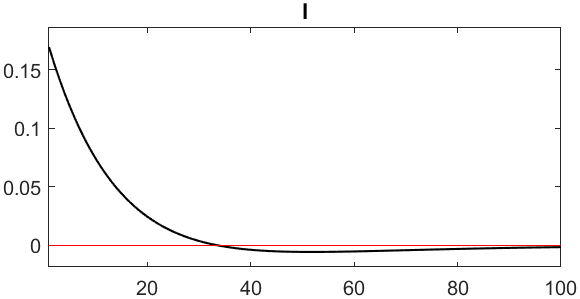
\includegraphics[scale=1]{I.png}
    \label{fig:fig1}
\end{figure}
\vspace{1cm}
\begin{figure}[h!]
    \centering
    \caption{Consumption Response}
    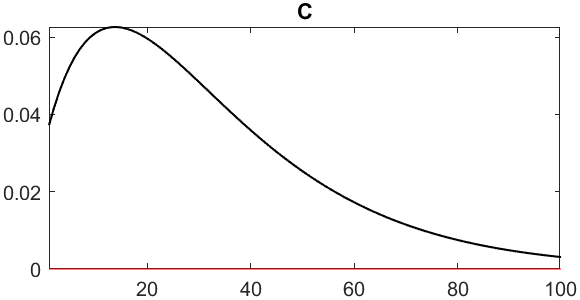
\includegraphics[scale=1]{C.png}
    \label{fig:fig2}
\end{figure}
\vspace*{1cm}
\begin{figure}[h!]
    \centering
    \caption{Labor Response}
    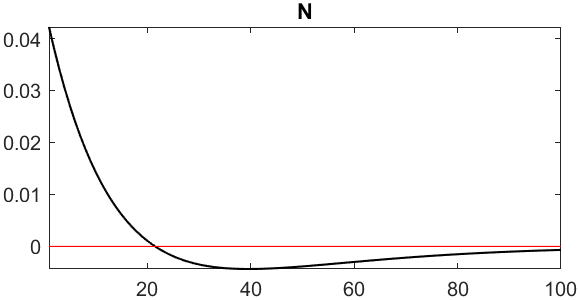
\includegraphics[scale=1]{N.png}
    \label{fig:fig3}
\end{figure}
\vspace*{1cm}
\begin{figure}[h!]
    \centering
    \caption{Capital Response}
    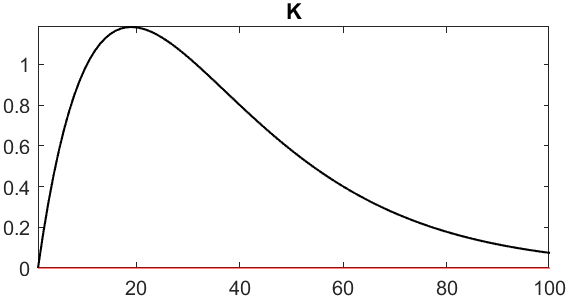
\includegraphics[scale=1]{K.png}
    \label{fig:fig4}
\end{figure}
\vspace*{1.2cm}
\begin{figure}[h]
    \centering
    \caption{Interest Rate Response}
    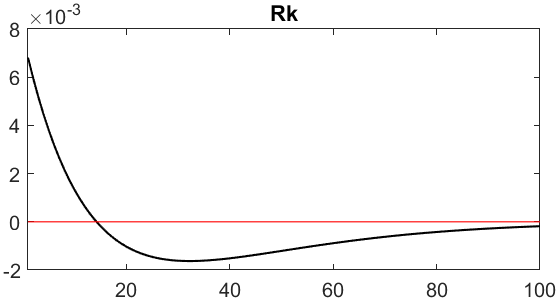
\includegraphics[scale=1]{Rk.png}
    \label{fig:fig5}
\end{figure}
\vspace*{1cm}
\begin{figure}[h!]
    \centering
    \caption{Wage Response}
    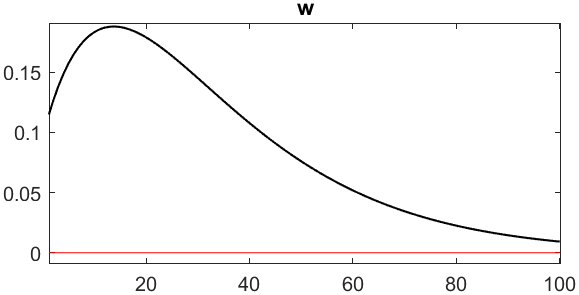
\includegraphics[scale=1]{w.png}
    \label{fig:fig6}
\end{figure}
\newpage
\begin{figure}[htpb]
    \centering
    \caption{Technology Response}
    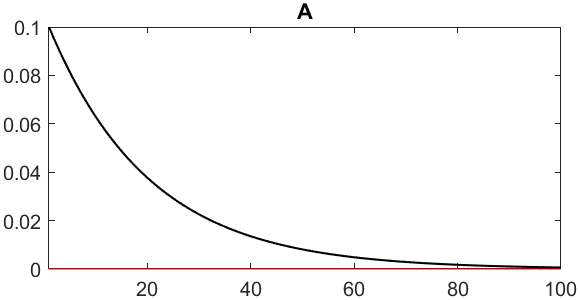
\includegraphics[scale=1]{A.png}
    \label{fig:fi8}
\end{figure}
\begin{figure}[htpb]
    \centering
    \caption{Output Response}
    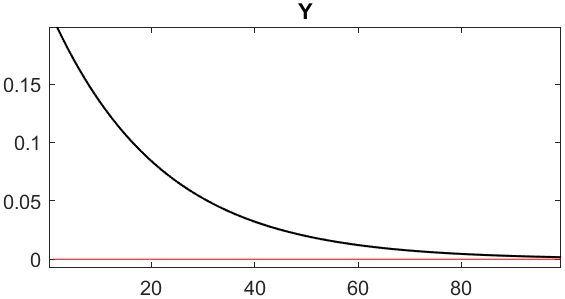
\includegraphics[scale=1]{Y.png}
    \label{fig:fig7}
\end{figure}
\newpage
\problem{5. Interpret}
Productivity, $\tilde{z}_t$, increases, leading to an immediate rise in the marginal product of labor and capital.\\
Wages $\tilde{w}_t$ and the rental rate on capital $\tilde{R_k}_{t}$ increase, reflecting the higher productivity.\\\\
Consumption, $\tilde{c}_t$, jumps due to the income effect of higher wages.\\
Investment, $\tilde{i}_t$, increases as firms seek to capitalize on the higher productivity by expanding their capital stock.\\\\
Labor supply is affected by two opposite effects; the substitution effect (working more due to higher wages) and the income effect (working less due to higher consumption).\\
Labor demand increases due to higher productivity, leading to an increase in employment, $\tilde{N}_t$ and wages $\tilde{N}_t$.\\\\
The capital stock $\tilde{k}_t$ grows over time as investment continues, leading to an expanded productive capacity of the economy.\\
Output $\tilde{Y}_t$ increases immediately due to higher productivity.\\\\
Over time, as the shock fades out, the output initially reaches its peak and then begins to decrease. This decrease in output leads to a decrease in demand for labor and capital, resulting in lower wages and interest rates. This, in turn, affects the supply side, leading to a further decrease in output, creating a vicious cycle of continued decline.
%%%%%%%%%%%%%%%%%%%%%%%%%%%%%%%%%%%%%%%%
%%%%%%%%%%%%%%%%%%%%%%%%%%%%%%%%%%%%%%%%
\end{document}






